% !TEX root = main21.tex
% Standalone addendum; the full paper remains in main2.tex, unchanged.
\documentclass[11pt]{article}
\usepackage[margin=1in]{geometry}
\usepackage[T1]{fontenc}
\usepackage{amsmath,amssymb}
\usepackage{microtype}
\usepackage{booktabs}
\usepackage{graphicx}
\usepackage{float}
\usepackage{xurl}
\usepackage[colorlinks=true,linkcolor=black,urlcolor=black]{hyperref}
\hypersetup{pdftitle={GROMM v1-4,3: Wider-grid calibration and VIX addendum}}

\newcommand{\E}{\mathbb E}
\newcommand{\Q}{\mathbb Q}

\title{\textbf{GROMM v1-4,3}\\[6pt]
  \large Wider-grid calibration and VIX\\
  Addendum to \emph{Generative Risk-neutral Option Market Models}}
\author{Magnus Wiese\qquad Hans Buehler\qquad Blanka Horvath}
\date{\today}

\begin{document}
\maketitle

This addendum reports only the new wider-grid experiment and its comparison
with the original GROMM v1. The main paper, \texttt{main2.tex}, is unchanged
and contains the model theory, proofs and earlier experiments. Here we
record the new calibration, fresh risk-neutral diagnostics and historical
VIX comparison; implementation details and reproducibility information
are collected in Appendix~\ref{app:wide-grid-details}.

% !TEX root = main21.tex
\section{A wider-grid GROMM v1 calibration and VIX}
\label{sec:wide-grid}
% Generated from completed reports; see metrics.json.
\newcommand{\WideVixMaeReduction}{75.33}
\newcommand{\WideCoreCoverage}{97.299}
\newcommand{\WideExplainedVariance}{75.87}
\newcommand{\WideOverallConditionalMedian}{1.98624}
\newcommand{\WideOverallMidpointMae}{0.56549}
\newcommand{\WideSquaredMean}{1.311}
\newcommand{\WideSquaredSe}{1.317}
\newcommand{\WideSquaredCiLow}{-1.270}
\newcommand{\WideSquaredCiHigh}{3.892}
\newcommand{\WideEntropyMean}{1.312}
\newcommand{\WideEntropySe}{1.318}
\newcommand{\WideEntropyCiLow}{-1.272}
\newcommand{\WideEntropyCiHigh}{3.896}


We consider a separately calibrated extension of the original GROMM v1,
\texttt{Gromm-v1-4,3}, intended
to improve coverage of the option wings relevant to variance swaps and VIX.
It has the same SDLV architecture: 25 daily expiries, 200 interior strikes,
5,000 direct state coordinates per date, and an independent 5\% Black
smoothing factor. Both the 100-node one-day template and the 100-node
25-day template are widened to NMS $[-4,3]$; the one-day grid is retained.
NMS denotes the main paper's regularized, ATM-volatility-scaled
log-moneyness coordinate; the original templates span $[-2.5,1.5]$.
The templates are merged into a common support as before. This changes the
strike coverage, not the model's 25-business-day maturity limit.
With the interior-node count held fixed, the wider support redistributes
strike resolution rather than adding state coordinates.

\subsection{Fresh calibration and market fit}

The new fit uses the same 891 dates, 3 January 2022--29 August 2025, and the
same upstream market-quality filters, but removes the final NMS quote cutoff.
All 3,141,110 remaining call and put intervals are used. Quotes with their
own expiry-specific NMS in $[-3.5,2.5]$ receive weight one; all others receive
weight $0.1$. This is not a claim to retain every raw exchange quote. Each
day's weighted loss is normalized by its sum of quote weights, and the
objective averages equally across days. The loss remains bid--ask excess
plus $0.05$ times absolute midpoint error, in half-spread units, together
with the original DLV cap penalty.

All daily model states were fitted from an ATM initializer, without
transferring the original trained weights. The complete original schedule
was run: 300 Adam epochs with cosine learning rate $0.02\to0.001$, followed
by 700 epochs with $0.005\to0.00005$, resetting Adam at the continuation
boundary. No VIX observations entered this objective.

\begin{table}[H]
\centering\small
\begin{tabular}{lrrrr}
\toprule
Fit / quote subset & Quotes & \% excess & Mean excess & Cond. mean \\
\midrule
Original v1, original range & 2,192,458 & 2.679\% & 0.03450 & 1.28797 \\
Wider fit, original range & 2,192,458 & 2.636\% & 0.03435 & 1.30311 \\
Wider fit, core & 2,465,684 & 2.701\% & 0.03484 & 1.28996 \\
Wider fit, wings & 675,426 & 31.635\% & 1.31125 & 4.14489 \\
Wider fit, all quotes & 3,141,110 & 8.923\% & 0.30930 & 3.46650 \\
Wider fit, 29 Aug. (all) & 4,190 & 15.012\% & 0.62411 & 4.15740 \\
\bottomrule
\end{tabular}
\caption{Static-fit errors beyond the bid--ask interval, in half-spread units. All statistics are unweighted quote-level summaries, not the weighted training objective. Conditional means include only quotes with positive excess. The original-range rows cover the same 2,192,458 retained quotes; the final row is a separate single-date summary.}
\label{tab:wide-static-fit}
\end{table}


Table~\ref{tab:wide-static-fit} separates the expanded quote universe from
the original comparison set. The wider fit covers \WideCoreCoverage\% of
the core quotes, whereas the downweighted wings remain appreciably harder
to fit. Across the full expanded universe, the conditional median excess
is \WideOverallConditionalMedian{} half-spreads and midpoint MAE is
\WideOverallMidpointMae{} half-spreads. The original-range rows should be
used when comparing static fit with the original GROMM v1;
the all-quote and single-date rows have different denominators.
Because grid coverage, quote scope and loss weights change together,
this experiment does not isolate the effect of grid width alone.

\subsection{Fresh diffusion estimation and risk-neutral audit}

The diffusion is re-estimated from the new historical fitted surfaces,
not transferred from GROMM v1. The estimator uses 710 exact one-session
pairs ending no later than 31 December 2024, with the same fixed-contract
alignment and Gaussian smoothing widths of one expiry and two strike nodes.
The eight-factor system, including the front-spot factor, captures
\WideExplainedVariance\% of the smoothed innovation variance. Thus the
29 August 2025 initial state is contemporaneously calibrated, while the
diffusion-estimation window ends before that date.
Appendix~\ref{app:wide-grid-factors} shows the new mean implied-volatility
surface, the saved innovation spectrum and all eight retained factor responses.

We use the same front-density bridge and recomputed risk-neutral DLV drift
as in the original model, with eight uniform substeps per day. From the
completed new state we generate 100,000 fresh paths arranged as 50,000
independent antithetic pairs. The 20-business-day trading universe is spot
plus 44 options, constructed from the new initial surface with the same
NMS and maturity rule as the main paper: eleven initially OTM calls or puts
at each of 5, 10, 15 and 20 business days, with cash strikes fixed thereafter.
Appendix~\ref{sec:wide-audit-definition} defines the reported statistics.
Both conditional policies are trained afresh, with whole paths and complete
pairs kept together in each fold. No old diffusion factors, simulated
populations or trained conditional policies are reused.

\begin{table}[H]
\centering\small
\begin{tabular}{rrrrrrr}
\toprule
$N$ & Max. $|z|$ & 99\% $|z|$ & $N_{2.576}$ & $N_5$ & $T_{\rm sqr}$ & $T_{\rm ent}$ \\
\midrule
570 & 2.426 & 2.118 & 0 & 0 & 0.995 & 0.995 \\
\bottomrule
\end{tabular}
\caption{Fresh GROMM v1-4,3 restricted-universe $\Q$ audit: 100,000 paths, 50,000 antithetic pairs, 20 business days, spot plus 44 options; eight factors and eight steps per day. The statistics and colour conventions are those of Appendix~\ref{sec:wide-audit-definition}.}
\label{tab:wide-q-audit}
\end{table}


None of the 570 day--instrument coordinates exceeds $2.576$ standard errors.
The squared policy's out-of-fold mean and pair-based standard error are
$(\WideSquaredMean,\WideSquaredSe)\times10^{-9}$ daily spot units, with 95\%
interval $[\WideSquaredCiLow,\WideSquaredCiHigh]\times10^{-9}$.
For the entropy policy the corresponding values are
$(\WideEntropyMean,\WideEntropySe)\times10^{-9}$ and
$[\WideEntropyCiLow,\WideEntropyCiHigh]\times10^{-9}$.
Both intervals contain zero. These diagnostics are consistent with the
risk-neutral null for the tested instrument universe and policy class;
they are not a proof over all strategies. In particular, the wider model
has \emph{not} undergone the main paper's 25-day full-instrument-grid audit,
nor a separate test of every
new wing strike. No new physical-measure simulation audit is claimed here.

\subsection{Historical VIX comparison}

Figure~\ref{fig:wide-vix-comparison} compares the original and wider models
with the official Cboe closing VIX and a reconstruction from the filtered
market spreads supplied to SANOS. The discrete model series reprice the
same market-selected option strips, with observed bid cutoffs and the
same expiry interpolation. The analytic series instead use the model's
full-strike log-contract variance at those same two expiries.
Appendix~\ref{app:wide-grid-details} specifies the formulas and clocks.

\begin{figure}[H]
  \centering
  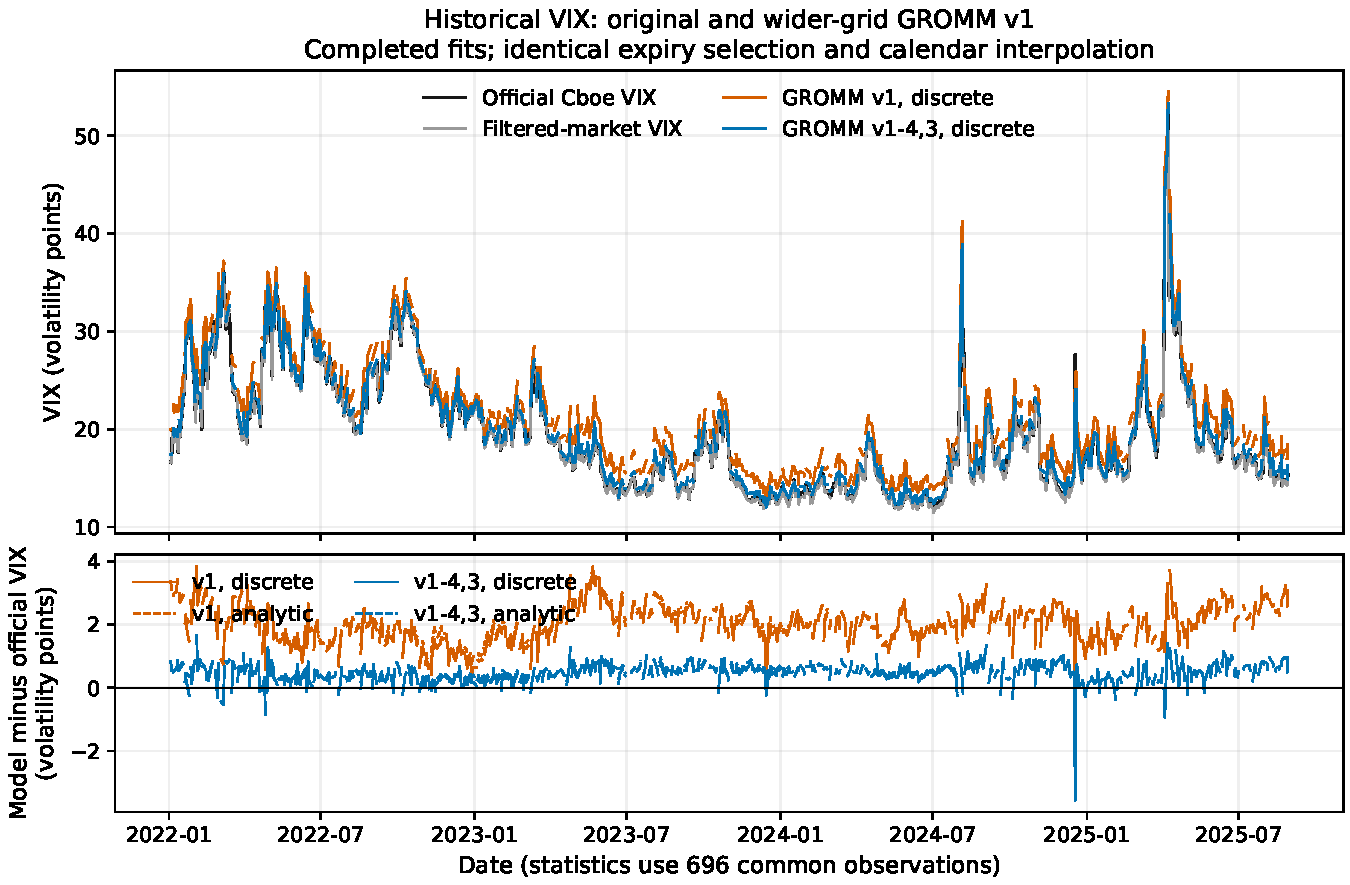
\includegraphics[width=\textwidth]{generated/wide_grid/gromm_v1_wide_vix.pdf}
  \caption{Historical VIX levels (top) and model errors relative to the
  official close (bottom). Orange denotes the original GROMM v1 and blue
  the completed GROMM v1-4,3 calibration. Solid model curves use the
  market-selected discrete strip; dashed error curves use the analytic
  full-strike variance swap. The grey top curve uses filtered market input
  spreads, not fitted SANOS prices. Statistics use the same 696 complete
  dates; missing model maturities are not extrapolated or filled in.}
  \label{fig:wide-vix-comparison}
\end{figure}

\begin{table}[H]
\centering\small
\begin{tabular}{lrrrrr}
\toprule
Series & Bias & MAE & RMSE & Corr. & 29 Aug. \\
\midrule
Raw-market strip & +0.028 & 0.142 & 0.265 & 0.99903 & 15.405 \\
Filtered SANOS input & -0.181 & 0.235 & 0.349 & 0.99873 & 15.197 \\
GROMM v1, discrete & +1.999 & 2.005 & 2.094 & 0.99446 & 18.434 \\
GROMM v1, analytic & +2.062 & 2.068 & 2.149 & 0.99481 & 18.432 \\
GROMM v1-4,3, discrete & +0.461 & 0.495 & 0.568 & 0.99848 & 16.314 \\
GROMM v1-4,3, analytic & +0.497 & 0.528 & 0.595 & 0.99853 & 16.318 \\
\bottomrule
\end{tabular}
\caption{Historical VIX comparison on the same 696 complete dates. Errors and the reference-date levels are in volatility percentage points; the benchmark is the official Cboe close (15.360 on 29 August 2025). Analytic values use the full-strike log contract at the same two expiries and the same calendar interpolation as the discrete strip, not direct evaluation at a different 30-day business maturity.}
\label{tab:wide-vix}
\end{table}


Discrete VIX MAE falls from 2.005 to 0.495 volatility points, a
\WideVixMaeReduction\% reduction on identical dates. The wider model's
analytic series has MAE 0.528 and RMSE 0.595; its remaining positive bias
shows that the wider calibration does not fully remove the discrepancy.
On the reference date the official close is 15.360, compared with 18.434
for the original discrete model and 16.314 for the wider discrete model.

There are 696 common model observations out of 891 fitted dates: on 186
dates a required Friday maturity exceeds the 25-business-day horizon, and
nine dates lack an eligible expiry bracket. The raw-market and filtered-input
reconstructions have 882 observations individually; Table~\ref{tab:wide-vix}
restricts them to the same 696 dates as the models. This is a historical
comparison of contemporaneously calibrated surfaces, not an out-of-sample
VIX forecast or a fit to VIX. Although the implemented discrete formula
follows the Cboe strike-selection and interpolation rules, archived
OptionMetrics end-of-day quotes and zero curves do not reproduce Cboe's
synchronous inputs and intraday filtering. We therefore do not claim an
exact reconstruction of the published closing tick.


\clearpage
\appendix
\begingroup
\small
% !TEX root = main21.tex
\section{Wider-grid calibration and VIX implementation}
\label{app:wide-grid-details}

\subsection{State representation and checks}
The wider model has 200 interior strikes plus two boundary nodes; the
boundary levels remain one half of the smallest interior strike and one
and a half times the largest. All 25 expiries share that support on a given
historical date. The support floats between historical dates but cash
strikes remain fixed within a simulated path and within each historical
one-session alignment. The DLV-squared parameterization retains minimum
$10^{-4}$ and upper cap $9$, with the original log-space barrier. The
completed fit's largest DLV-squared value is $6.319$, with no coordinate
at the cap. Across all historical states, independent float64 reconstruction
has minimum probability $3.46\times10^{-24}$ and maximum mass/forward errors
below $4.3\times10^{-14}$.

Training uses float32 as in the baseline. Its finite-difference point-mass
initializer has a small signed boundary roundoff of about
$-1.79\times10^{-7}$. Such checkpoints are accepted only when negative
mass is bounded by that initializer's roundoff and independent float64
reconstruction passes strict positivity, unit-mass and unit-forward checks.
The Q simulation and its initial-state reconstruction use float64.
This numerical calibration check is separate from the dynamic drift tests.

\subsection{Diffusion and audit conventions}
\label{sec:wide-audit-definition}
Historical log-DLV changes are aligned at fixed expiry and cash strike;
the endpoint surface is interpolated at origin relative strike divided by
the realized gross spot return. A nodewise physical AR fit removes the
conditional mean before smoothing and the joint spot/surface PCA.
For the Q audit the drift is recalculated from the density recursion,
not obtained by setting the empirical physical drift to zero.
The simulator retains the paper's log-Euler step and its exceptional
relative-drift taming threshold $0.5$; it is not an exact finite-step
martingale correction. The independent 5\% Black factor has zero Q drift.
The two conditional objectives, fold construction and spot normalization
are those of the main paper; each
fold uses a 30-epoch affine warm start and 30-epoch affine-plus-deep fit,
with two width-32 SiLU layers, learning rate $10^{-3}$ and batch size 2,048.
The simulation seed is 20261024. Constant physical risk prices are also
re-estimated, but the new reported path diagnostics are under Q only.

For each live day--instrument coordinate, the return is
$R_{p,n}^i=(V_{p,n+1}^i-V_{p,n}^i)/Z_{p,n}$, where $Z$ is pre-step spot
and $V^i$ is spot or an option price. The unconditional score is its sample
mean divided by the standard error computed across 50,000 antithetic-pair
averages. Table~\ref{tab:wide-q-audit} reports the maximum and empirical
99th percentile of $|z|$ over the 570 coordinates, together with counts
$N_c$ for $|z|>c$. These coordinatewise thresholds are not family-wise
$p$-values.

Conditional policies use current Brownian-factor histories, log spot,
live log option-price-to-spot ratios, time and remaining maturities. For
an action $a(X)$, write $r=a(X)^\top R$. The squared objective maximizes
the training mean of $r-\tfrac12\lVert a\rVert^2-\tfrac12r^2$; the entropy
objective minimizes $\log\operatorname{mean}\exp(-r+\tfrac12\lVert a\rVert^2)$.
Complete antithetic pairs are split into two equal folds; input
standardization and action fitting use only the training fold, and each
frozen policy is evaluated on the other fold. The folds are then exchanged.
For either objective, the reported $T$ is the mean out-of-fold daily
portfolio return divided by its pair-based standard error, after averaging
over the 20 days within each path. The main paper's per-test colour rule is
black for $|T|\leq1.96$, orange for $1.96<|T|\leq2.576$ and red above
$2.576$. Both new conditional statistics are therefore black.

\subsection{Market-selected discrete variance}
For each eligible expiry let $D_T$ be the discount factor, $F_T$ the
put--call-parity forward, $K_0$ the greatest available strike not exceeding
$F_T$, and $O_T(K)$ the selected OTM midpoint price (the average of call
and put prices at $K_0$). The Cboe total-variance formula is
\begin{equation}\label{eq:wide-vix-strip}
  v_T^{\mathrm{strip}}
  =\frac{2}{D_T}\sum_i\frac{\Delta K_i}{K_i^2}O_T(K_i)
   -\left(\frac{F_T}{K_0}-1\right)^2.
\end{equation}
Interior $\Delta K_i$ are half the neighbouring-strike difference; endpoints
use the adjacent-strike difference. Selection walks outward from $K_0$,
omits zero-bid contracts and stops after two consecutive zero bids on each
side. Friday expiries strictly between 23 and 37 calendar days are selected
with their AM/PM settlement convention. For minute counts $N_1<N_{30}<N_2$,
\begin{equation}\label{eq:wide-vix-interpolation}
  \mathrm{VIX}
  =100\sqrt{\frac{N_{365}}{N_{30}}\left[
    \frac{N_2-N_{30}}{N_2-N_1}v_{T_1}
    +\frac{N_{30}-N_1}{N_2-N_1}v_{T_2}\right]},
\end{equation}
where $N_{30}=43,200$ and $N_{365}=525,600$.
These conventions follow the \href{https://cdn.cboe.com/resources/vix/VIX_Methodology.pdf}
{Cboe VIX methodology}, pp.~2--7.

The model replaces only the option prices in
\eqref{eq:wide-vix-strip}; the observed raw bid cutoffs, forward, $K_0$,
discount factors, contracts and interpolation times are shared by both
GROMM variants. No fictitious model bid/ask quotes are introduced.
Filtered-market VIX uses the synthetic call-equivalent bid/ask midpoints
passed to SANOS, including parity conversion for puts, not fitted option
prices. Since preprocessing has removed zero bids, the filtered-strip
calculation respects the observed raw-book cutoffs, then computes its own
forward, $K_0$ and strike quadrature on the surviving input quotes.

\subsection{Analytic full-strike variance}
For the forward-normalized mixture $S_T/F_T=s_JB_T$, with probabilities
$p_j(T)$ on positive support $s_j$ and independent mean-one Black factor
of business-time variance $0.05^2\tau_b(T)$, the model gives
\begin{equation}\label{eq:wide-analytic-variance}
  v_T^{\mathrm{analytic}}
  =-2\E^\Q\!\left[\log(S_T/F_T)\right]
  =-2\sum_jp_j(T)\log s_j+0.05^2\tau_b(T).
\end{equation}
This is the full-strike log-contract/variance-swap quantity, not a discrete
VIX strip. We substitute these two expiry values into
\eqref{eq:wide-vix-interpolation}; a direct 30-calendar-day model evaluation
has a different maturity convention and is not used in
Table~\ref{tab:wide-vix} or Figure~\ref{fig:wide-vix-comparison}.

Calendar time is measured from 16:15 New York to 09:30 for AM settlement
or 16:00 for PM settlement. Model business time uses the NYSE session
calendar divided by 252 and the implementation's $0.8$-day AM subtraction.
Fractional model maturities interpolate adjacent daily densities. Discount
factors use the cached OptionMetrics zero curve with linear rate
interpolation, not Cboe's Treasury spline. No maturity beyond 25 business
days is extrapolated. These clock and input differences are retained in
the reported comparisons, not calibrated away by a VIX rescaling.

\subsection{Reproducibility}
The fresh calibration is run by
\path{quantdata/sdlv/daily/wide_fit.py}; the Q audit by
\path{quantdata/sdlv/daily/wide_audit.py}; and the VIX calculations by
\path{quantdata/sdlv/daily/vix_comparison.py} and
\path{quantdata/dysanos/filtered_vix.py}, using the shared formula in
\path{quantdata/vixdata/formula.py}.
The source for the new tables and figure is
\path{quantdata/sdlv/daily/paper_wide_grid.py}.
The retained \path{generated/wide_grid/metrics.json} records the completed
fit and audit, source paths and SHA-256 hashes; the accompanying
\path{vix_series.csv} supplies the plotted observations. Large training
data, checkpoints and simulation chunks remain outside the Git tree.
This experiment uses training run \path{20261023-kVyePV} and Q-audit
run \path{q-audit-20261024-4mkznc}. The VIX and Q results are checked
to refer to the identical final 1,000-epoch checkpoint; no interim VIX
snapshot is used in this addendum.

\endgroup

\clearpage
% !TEX root = main21.tex
\section{Mean volatility surface and new PCA factors}
\label{app:wide-grid-factors}
\newcommand{\WidePcaNinetyRank}{25}


\subsection{Mean and reference-date implied volatility}

Figure~\ref{fig:wide-mean-iv} shows the arithmetic mean of the wider model's
Black implied-volatility surfaces over all 891 fitted dates, with equal
weight per date. Each surface is evaluated on the same NMS $[-4,3]$ and
1--25-business-day grid, using that date's market ATM volatility scale.
This is a mean of implied volatilities, not the implied volatility of an
averaged price surface, nor an average of the DLV parameters. The right
panel is the 29 August 2025 fitted state used for the factor illustrations.
Neither panel averages simulated paths. Both include the 5\% Black
smoothing component and use business-time annualization.

\begin{figure}[H]
  \centering
  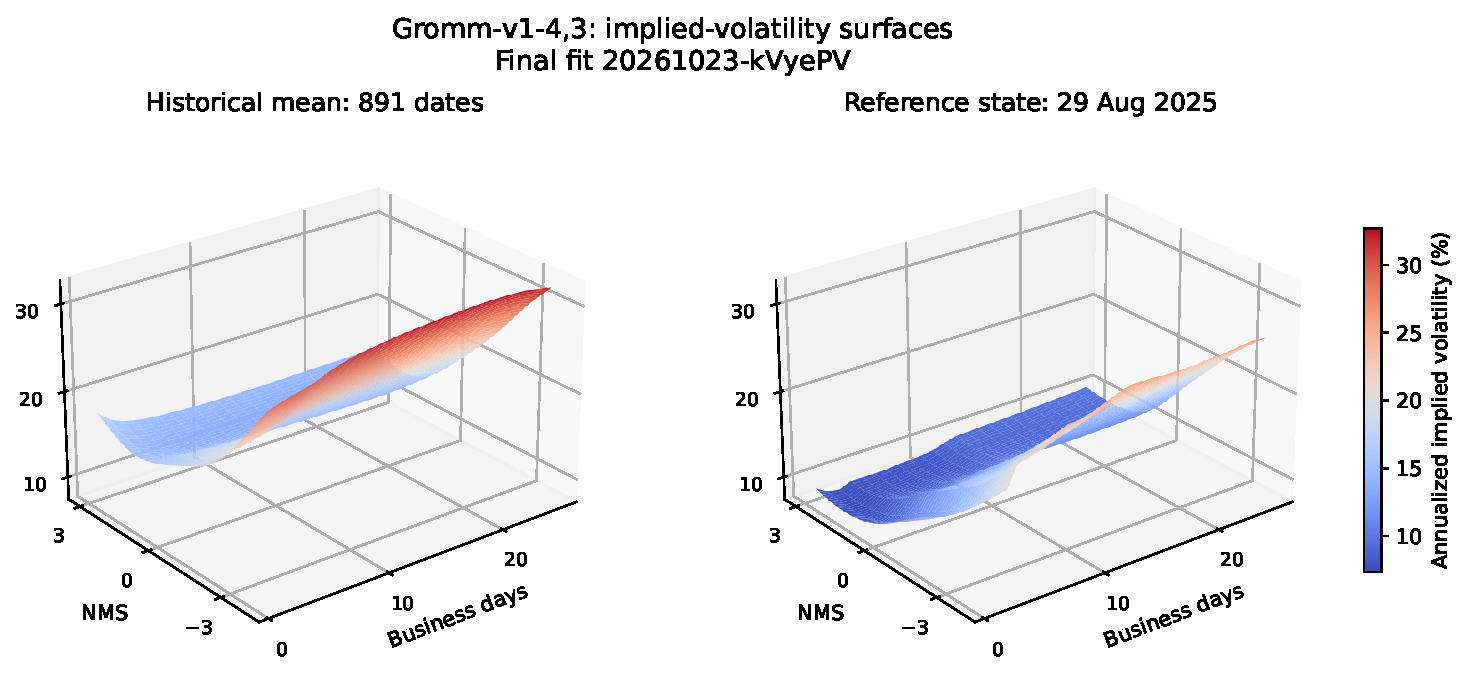
\includegraphics[width=\textwidth]{generated/wide_grid/mean_and_reference_iv.pdf}
  \caption{GROMM v1-4,3 annualized implied volatility in percent: historical
  equal-date mean (left) and reference-date state (right). Both panels use
  identical vertical and colour scales. Date-specific NMS alignment prevents
  the historical mean from mixing different standardized strikes. These are
  model surfaces over the displayed grid, including downweighted wings, not
  a claim of observed quote coverage at every plotted point.}
  \label{fig:wide-mean-iv}
\end{figure}

\subsection{Innovation spectrum}

The new factor system is the one saved by the completed wider-grid Q audit,
estimated from 710 fixed-contract historical pairs ending on 31 December
2024. The first direction is aligned to the front-spot innovation; the
remaining seven retained directions are PCs of the smoothed log-DLV
innovations after removing their spot projection. These are not PCs of
implied-volatility levels. Figure~\ref{fig:wide-pca-spectrum} reports the
spot-loading power followed by the residual covariance eigenvalues, each
divided by total smoothed innovation variance. The eight retained factors
explain \WideExplainedVariance\%; the first 90\% crossing is rank
\WidePcaNinetyRank. Eigenvalues beyond rank eight are shown for context;
those additional directions were not used in the reported Q audit.

\begin{figure}[H]
  \centering
  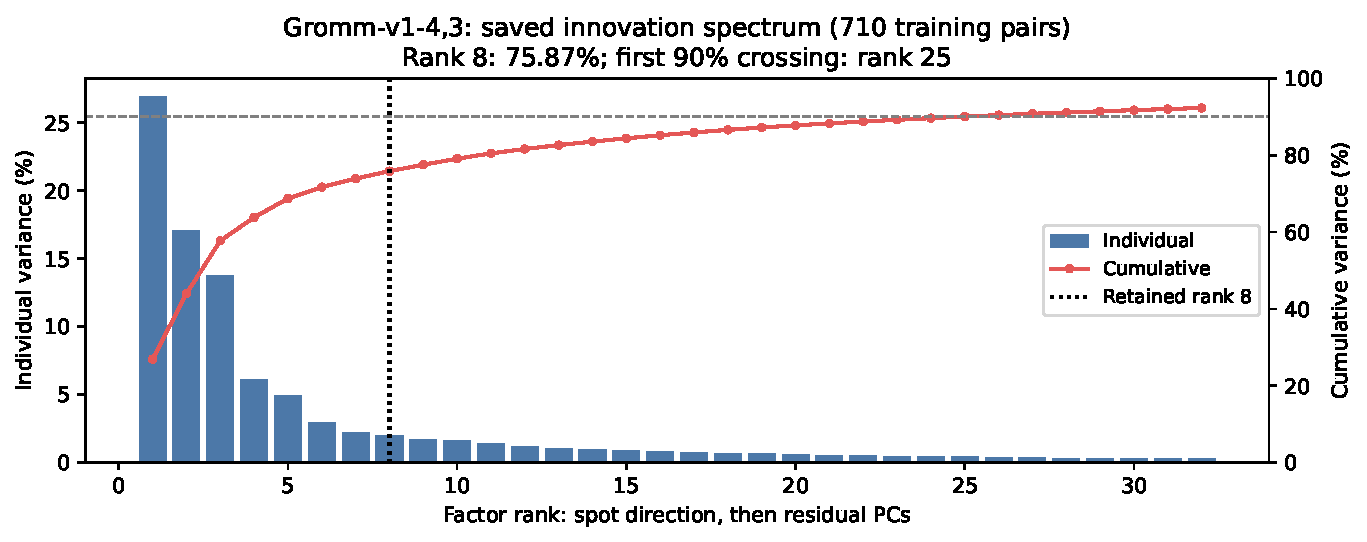
\includegraphics[width=0.94\textwidth]{generated/wide_grid/pca_explained_variance.pdf}
  \caption{New spot-oriented factor spectrum, using the saved wider-grid
  diffusion estimate. Blue bars show individual variance contributions;
  the red line is cumulative. The vertical dotted line marks the eight
  retained factors, not the rank needed to reach the horizontal 90\% line.}
  \label{fig:wide-pca-spectrum}
\end{figure}

\subsection{Implied-volatility responses of the retained factors}

At the reference-date state, each saved annualized loading $\xi_f$ is
mapped to an implied-volatility response by the same central daily shock
convention as the main paper:
\begin{equation}
  \Delta_f\sigma_{\rm imp}
  =\tfrac12\left[
    \sigma_{\rm imp}(\log\Sigma+\xi_f/\sqrt{252})
    -\sigma_{\rm imp}(\log\Sigma-\xi_f/\sqrt{252})\right].
\end{equation}
Only the future log-DLV-squared rows (days 2--25) are displaced. Spot,
the first-expiry state, and the reference-date NMS-to-strike map are held
fixed. Thus even for the spot-aligned factor this is its surface-loading
component, not a full joint spot/front-density simulation. There is no
drift or elapsed-time step in these illustrations; an equivalent measure
change leaves the illustrated diffusion directions unchanged.

\begin{figure}[H]
  \centering
  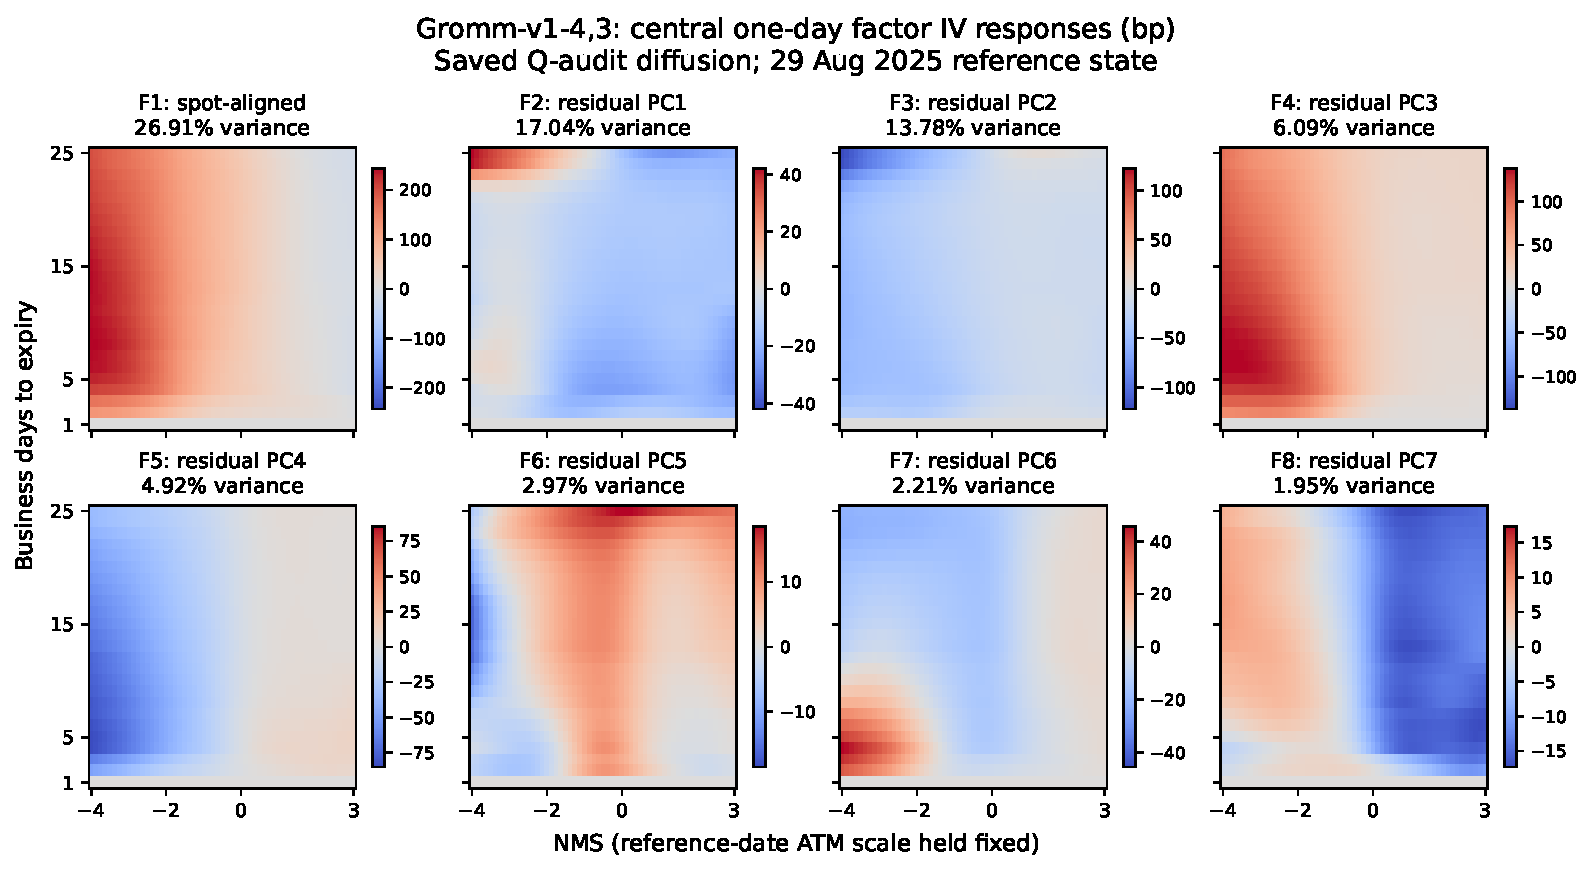
\includegraphics[width=\textwidth]{generated/wide_grid/pca_iv_responses.pdf}
  \caption{All eight new retained factors in IV coordinates. Each panel
  shows the central one-day-standard-deviation response in basis points of
  annualized IV ($1$ bp $=10^{-4}$), using its own symmetric colour scale.
  Panel percentages are contributions to total smoothed log-DLV innovation
  variance, not IV variance. F1 is spot-aligned; F2--F8 are residual PCs
  1--7. The one-day row is zero because its state is held fixed.}
  \label{fig:wide-pca-responses}
\end{figure}

The figures are regenerated by \path{quantdata/sdlv/daily/paper_wide_factors.py}.
Their plotted arrays and provenance are retained in
\path{generated/wide_grid/factor_surfaces.npz} and
\path{generated/wide_grid/factor_metrics.json}. Checkpoint identities,
reference-state reconstruction and retained variance are verified against
the same completed Q audit used in Table~\ref{tab:wide-q-audit}; no new
calibration or path simulation is performed to make these illustrations.


\end{document}
